\chapter{Introduction}
\label{c:introduction}
Particle physics research over the last century or so has provided us with our current basic understanding of
the fundamental particles that have made up the universe since its origin, and their interactions with each
other. This is summarised by the Standard Model (SM) of particle physics, which has been developed
incrementally in recent decades and has stood up well to scientific scrutiny. The Large Hadron Collider (LHC)
at the Organisation Europ\'{e}enne pour la Recherche Nucl\'{e}aire (CERN) near the Swiss city of Geneva
(Figure~\ref{fig:LHC_map}) was constructed with the aim of investigating the SM. Areas of current interest
including electroweak symmetry breaking, the Higgs mechanism and physics beyond the SM (BSM) such as
supersymmetry (explained in further detail in Section~\ref{c:the_standard_model}), require the acceleration of
particles to high energies (of the order of several TeV). The start of data-taking from proton-proton
collisions at the LHC in 2009 ushered in a new era in terms of energies at particle colliders, taking over as
the highest energy particle collider from the TeVatron at Fermilab. In 2010 and 2011 the LHC collected data at
a centre of mass energy of 7\TeV (5.1\fbinv), followed by 8\TeV (21.8\fbinv) in 2012 and currently in 2015
after the first long shutdown at 13\TeV.

The Compact Muon Solenoid (CMS) general-purpose detector is one of the four main detectors located around the
LHC (the others being ATLAS, LHCb and ALICE), approximately 100\m below ground level.

\begin{figure}[!hbtp]
   \centering
     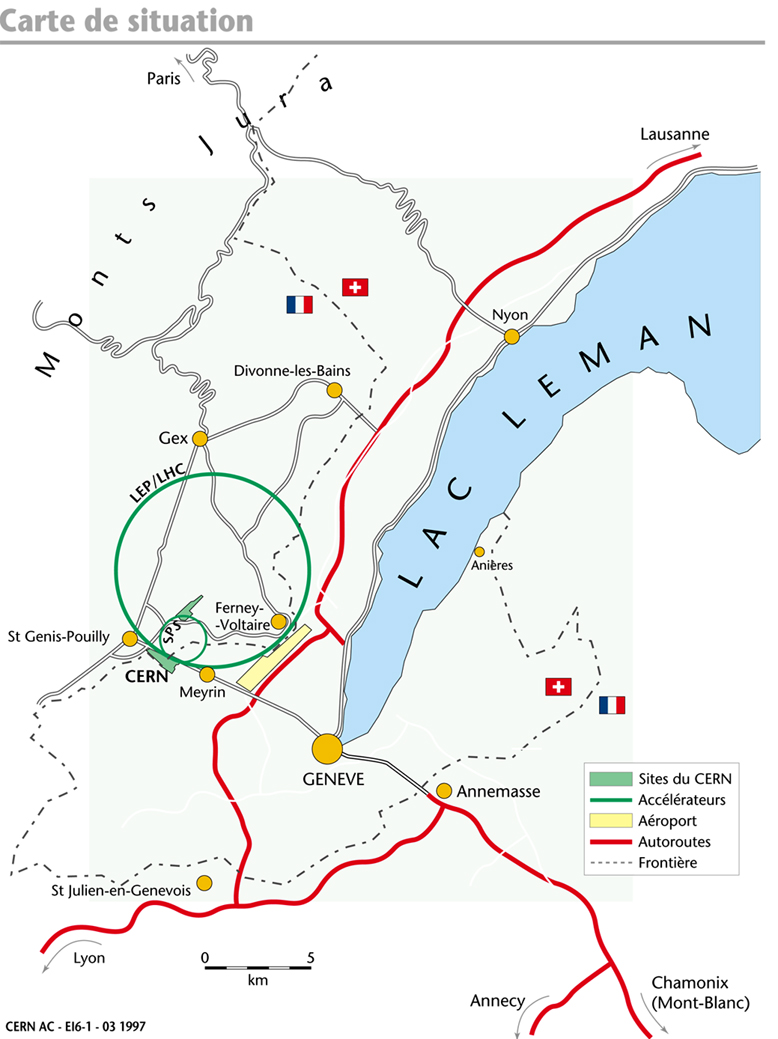
\includegraphics[width=0.6\textwidth]{Chapters/01_Introduction/Images/lhc-pho-1997-169.jpg}\\
     \caption{Map of LHC location.}
     \label{fig:LHC_map}
\end{figure}

This thesis presents an analysis based on the full proton-proton collision data from the CMS experiment in
2011 and 2012. The analysis investigates the top-antitop (\ttbar) differential cross section with respect to
global level event variables, specifically in semileptonic \ttbar decays in the electron+jets and muon+jets
channels. This investigation is motivated primarily by the importance of understanding \ttbar events, since
they are a significant background in many new physics analyses. The understanding of QCD and event generators
that studies such as this provide is also helpful for other physics analyses. Furthermore, rare Standard Model
processes such as $\ttbar + W\rightarrow l\nu$ or $\ttbar + Z\rightarrow \nu\bar{\nu}$ would appear in \met
distribution tail, and $\ttbar + X$ where $X$ is massive would appear in the \HT and \st distributions. There
are also possible new physics scenarios such as stop pair production, $\tilde{t}\bar{\tilde{t}} \rightarrow
t\tilde{\chi_0} \bar{t}\bar{\tilde{\chi_0}}$ which could show hints of dark matter.

The work presented here was carried out in collaboration with Emyr Clement, L{}ukasz Kreczko, Sergey Senkin
and Philip Symonds under the supervision of Professors Joel Goldstein and Greg Heath. The main contribution of
the author to these studies lay in development of the C++ and Python software frameworks and scripts used in
the analyses. Related to this, maintaining up-to-date particle object definitions, corrections, efficiencies
and prescription recommendations from working groups within CMS was a large component of the author's work. In
terms of the technical workflow employed, the author was heavily involved in producing n-tuples from the
analysis-ready AOD data format, running the software to perform the prescribed analysis methods, and running
final scripts on the output ROOT data to perform the final calculation and to produce results plots and
tables. Particular areas of focus regarding physics included synchronisation of the event selection,
comparison of distribution shapes between 7\TeV and 8\TeV data, and implementing aspects of the analyses such
as selection criteria, \btagging and jet energy resolution.

Chapters~\ref{c:CMS_Detector} and \ref{c:CMS_computing_and_offline} describe the LHC and the CMS detector,
including information about the object reconstruction process based on detector readout, to represent
particles produced in collisions. Chapter~\ref{c:the_standard_model} provides an overview of the Standard
Model theory and some of its shortcomings, followed by a review of physics of the top quark at the LHC in
Chapter~\ref{c:top_physics_at_the_lhc}. A small study investigating the \btagging algorithms used in CMS is
described in Chapter~\ref{c:b_tagging_study}, and the main \ttbar differential cross section analysis is then
covered in Chapters~\ref{c:Differential_Cross_Section:data_simulation_and_selection},
\ref{c:Differential_Cross_Section:fitting_unfolding_and_measurement}
and~\ref{c:Differential_Cross_Section:systematics_and_results}. To conclude, Chapter~\ref{c:summary} contains
a summary and outlook to the future. Additional data, tables and plots from the presented analyses are given
in Appendices~\ref{ac:b_tagging_plots} and \ref{ac:ttbar_diff_cross_section_analysis}. Finally, an addendum
describing the brief continuation of work from the author's MSc in testing a readout chip for the CMS strip
tracker is outlined in Appendix~\ref{ac:cbc}.

From the outset, natural units are used throughout this thesis, unless otherwise specifed, so that
\begin{equation}
\hbar = c = 1,
\end{equation}
meaning that mass, momentum and energy all have the same units of electronVolts (eV).